\documentclass{thesis}

\newcommand{\thesistitle}{TODO TITLE}
% Angestrebter Doktorgrad: med (Dr. med.), dent (Dr. med. dent.) oder schum (Dr. sc. hum.)
\newcommand{\thesisdegree}{med}
\newcommand{\thesisdegreephrase}{%
  \ifdefstring{\thesisdegree}{dent}{des Doktorgrades in der Zahnheilkunde}{%
  \ifdefstring{\thesisdegree}{schum}{des Doctor scientiarum humanarum (Dr.\,sc.\,hum.)}{%
  des medizinischen Doktorgrades}}}
% KI-basierte Hilfsmittel verwendet? \kiverwendettrue: Erklärung (Muster 11 a) +
% Anhang (Muster 11 b); \kiverwendetfalse: Nichtverwendungserklärung (Muster 12)
\newif\ifkiverwendet
\kiverwendettrue
% Sprache der Arbeit: de (deutsch) oder en (englisch). Laut Abfassungsrichtlinien
% gibt es genau eine Zusammenfassung (max. 2 Seiten, ohne Abkürzungen, Zitate,
% Abbildungen, Tabellen); kein zusätzliches Abstract. Nur bei englischer Arbeit
% kommt zum englischen Summary zusätzlich eine deutsche Zusammenfassung.
\newcommand{\thesislanguage}{en}

\usepackage{mathpazo}  % font: palatino vs computer modern
\usepackage{lipsum} % used to fill random text in sections
\usepackage{tikz} % used for sample figure

\newenvironment{dedication}
  {%\clearpage           % we want a new page          %% I commented this
   \thispagestyle{empty}% no header and footer
   \vspace*{\stretch{1}}% some space at the top
   \itshape             % the text is in italics
   \raggedleft          % flush to the right margin
  }
  {\par % end the paragraph
   \vspace{\stretch{3}} % space at bottom is three times that at the top
   \clearpage           % finish off the page
  }

\begin{document}

    % Titlepage (empty pagestyle)
    % Contains titlepage, empty page, "Prodekan + Doktorvater", empty page
    \pagestyle{empty}
    \pagenumbering{gobble}
    %\begin{titlingpage*}
\begin{center}

    Aus dem/der \textit{TODO: institution name} \\

    (Vorstand: \textit{TODO: board members}) \\
    Abteilung \textit{TODO: department} \\
    %\todo{Aktualisieren!}
    (Leiter: \textit{TODO: department head})

    \vfill
    
    %\rule{\linewidth}{0.5mm} \\
    %\vspace*{0.4cm}
    {\Huge \scshape {\thesistitle \par}} % Title is defined in main.tex
    %\vspace*{0.2cm}
    %\rule{\linewidth}{0.5mm} \\
    %\vspace*{1.6cm}

    \disclosure{TODO: \textit{The format of the dissertation might change in the future, so you should always check that this template is in agreement with the latest version provided by the medical faculty: \textcolor{blue}{\href{https://www.medizinische-fakultaet-hd.uni-heidelberg.de/fakultaet/akademische-laufbahn/promotion/promotion-zum-dr-sc-hum/schreiben-der-dissertation}{Composition Guidelines}}. You should remove this disclosure from the file "titlepage.tex" once you have checked that you are using the correct format.}}

    \vfill

    Inauguraldissertation \\
    zur Erlangung \thesisdegreephrase \\ % Doktorgrad wird in main.tex über \thesisdegree gesetzt
    an der \\
    Medizinischen Fakultät Heidelberg \\
    der \\
    Ruprecht-Karls-Universität 

    \vfill

    vorgelegt von \\
    \textit{TODO: name of doctoral candidate} \\
    aus \\
    \textit{TODO: city of birth, and country} \\
    \bigskip
    \textit{TODO: year of submission}

\end{center}

\newpage
\null\newpage
\vspace*{\fill}
 
% Den/die zum Zeitpunkt der Einreichung amtierende/n Dekan/in auf der Seite der
% Medizinischen Fakultät Heidelberg nachsehen, nicht aus einer älteren Arbeit übernehmen.
\noindent Dekan: \textit{TODO: Prof. Dr. ... (aktuelle/n Dekan/in prüfen, ggf. „Dekanin:“)} \\
Doktorvater/Doktormutter: \textit{TODO: name of the official supervisor} 

\newpage
\null\newpage
    \begin{dedication}
\usefont{T1}{LobsterTwo-LF}{bx}{it}
TODO, write here your dedication (one line), or delete the entry in main.tex.
\end{dedication}

    \cleardoublepage
    \tableofcontents
    \cleardoublepage

    \pagestyle{fancy}
    \setcounter{tocdepth}{2}
    \frontmatter
    \setcounter{page}{1}
    % Add acronyms from file (_Acronyms.tex) and add to table of contents
    {
    \chapter*{Acronyms}
    \renewcommand{\leftmark}{ACRONYMS}
    \renewcommand{\rightmark}{ACRONYMS}
    \addcontentsline{toc}{chapter}{Acronyms}
    
    \markboth{Acronyms}{} % Sorgt dafür, dass header für Kapitel Abstract stimmt.(http://www.weinelt.de/latex/markboth.html9
    
    \begin{acronym}[MMMMMMMM]
        \acro{SA}{Sample Acronym}
    \end{acronym}
}

    % Add list of figures and list of tables
    \newpage
    \phantomsection
    \addcontentsline{toc}{chapter}{List of Figures}
    \listoffigures
    \cleardoublepage
    \phantomsection
    \addcontentsline{toc}{chapter}{List of Tables}
    \listoftables

    \mainmatter
    % % Main Body of thesis
    \chapter{Introduction}
\label{chap:introduction}

\lipsum[1]

    \section{Motivation} 
\label{sec:introduction:motivation}

This is an example of a simple acronym that will be included in the list of acronyms: \ac{SA}. This is an example of a citation in the Harvard style required by the faculty~\citep{platzhalter}; see refs.bib for the placeholder entry.

This is an example of a figure (Fig.~\ref{fig:motivation:sample_figure}) that is automatically listed in the list of figures:

\begin{figure}[htbp]
    \centering
    \begin{tikzpicture}[scale=1.5]
        \draw[->] (-0.5,0) -- (5,0) node[right] {$x$};
        \draw[->] (0,-1.5) -- (0,1.5) node[above] {$y$};
        \draw[domain=0:4.5, smooth, variable=\x,blue] plot (\x, {sin(\x r)}) node[right] {$f(x) = \sin(x)$};
        \foreach \x in {1,2,3,4}
            \draw (\x cm,1pt) -- (\x cm,-1pt) node[anchor=north] {$\x$};
        \foreach \y in {-1,1}
            \draw (1pt,\y cm) -- (-1pt,\y cm) node[anchor=east] {$\y$};
    \end{tikzpicture}
    \caption{Graph of $y = \sin(x)$.}
    \label{fig:motivation:sample_figure}
\end{figure}

This is an example of a table (Tab.~\ref{tab:motivation:sample_table}) that is automatically included in the list of tables:

\begin{table}[htbp]
    \centering
    \begin{tabular}{|c|c|c|c|c|}
        \hline
        \rowcolor{lightgray}
        Measurement & Unit & Value 1 & Value 2 & Value 3 \\
        \hline
        Length & mm & 12.3 & 12.8 & 11.9 \\
        Temperature & \degree C & 36.5 & 36.8 & 36.4 \\
        \hline
    \end{tabular}
    \caption{Sample table with random values.}
    \label{tab:motivation:sample_table}
\end{table}

\disclosure{Important disclosure}{This is an example of a "disclosure" that can be used to disclose relevant information or highlight important text.}

\researchquestion{1}{This an example of a research question box, that can be used to highlight the statements of your research questions.}

    \section{Background} 
\label{sec:introduction:background}

\lipsum[1-3]
    \section{Related Work} 
\label{sec:introduction:related_work}


\lipsum[1-3]
    \section{Objectives and Contributions}
\label{sec:introduction:objectives}


\lipsum[1-3]

    \section{Outline} 
\label{sec:introduction:outline}


\lipsum[1-3]
        
    \chapter{Materials and Methodology}
\label{chap:materials_and_methods}

\lipsum[1]   

    \section{TODO TITLE} 
\label{sec:methods:methods_one}

\lipsum[1-3]
    
    \chapter{Results}
\label{chap:results}

\lipsum[1]

    \section{TODO TITLE}
\label{sec:results:results_one}

\lipsum[1-3]
    \chapter{Discussion}
\label{chap:discussion}

\lipsum[1]   

    \section{TODO TITLE} 
\label{sec:discussion:diss_one}

\lipsum[1-3]

    \ifdefstring{\thesislanguage}{en}{%
        \chapter{Summary}


\lipsum[1-5]
        \chapter{Zusammenfassung}

\lipsum[1-5]
    }{%
        \chapter{Zusammenfassung}

\lipsum[1-5]
    }
    
    \clearpage
    \phantomsection
    \addcontentsline{toc}{chapter}{Bibliography}
    \markboth{Bibliography}{Bibliography}
    \bibliography{refs} % In overleaf you can link to Zotero. Go to "new file"->"From Zotero"

    \chapter*{Own Contributions}
\addcontentsline{toc}{chapter}{Own Contributions and Publications}
\markboth{Own Contributions and Publications}{Own Contributions and Publications}
\label{chap:contributions}

This chapter gives an overview of my contributions in distinction to team efforts.


\section*{Own share in data acquisition and data analysis}
\phantomsection
\addcontentsline{toc}{section}{Own share in data acquisition and data analysis}
\label{sec:own-data-acquisition}

    
\lipsum[1]

\paragraph{Own share in Data Acquisition.}
\lipsum[1]  

\paragraph{Own share in Data Analysis.}
\lipsum[1] 
        
        

\section*{Own Publications}
\addcontentsline{toc}{section}{Own Publications}
\label{sec:own-publications}

In this section, all publications that I was a part of and contributed to during my Ph.D. work are listed. It is subdivided into \textit{First Authorships} and \textit{Co-Authorships}.
\hfill \break

\subsection*{First Authorships - Peer Reviewed International Journal Publications} \label{sec:publications:peer_reviewed_journal_first}

\begin{itemize}
    \item[] TODO: eigene Publikation im Format Autor:innen, Jahr, Titel, Zeitschrift, DOI (oder Abschnitt löschen, falls keine).
\end{itemize}

\subsection*{First Authorships - Peer Reviewed International Conference Publications} \label{sec:publications:peer_reviewed_conf_first}

\begin{itemize}
    \item[] TODO: eigene Publikation im Format Autor:innen, Jahr, Titel, Zeitschrift, DOI (oder Abschnitt löschen, falls keine).
\end{itemize}

\subsection*{Co-Authorships} \label{sec:publications:other_co}

\begin{itemize}
    \item[] TODO: eigene Publikation im Format Autor:innen, Jahr, Titel, Zeitschrift, DOI (oder Abschnitt löschen, falls keine).
\end{itemize}


    \chapter*{Appendix}
\addcontentsline{toc}{chapter}{Appendix}

\lipsum[1-3]

    \pagestyle{plain}
    % Lebenslauf: laut Abfassungsrichtlinien optional, steht nach dem Anhang.
    % figures/CV.pdf durch den eigenen Lebenslauf ersetzen oder diesen Block
    % auskommentieren, wenn kein Lebenslauf eingebunden werden soll.
    \phantomsection
    \addcontentsline{toc}{chapter}{Curriculum Vitae}
    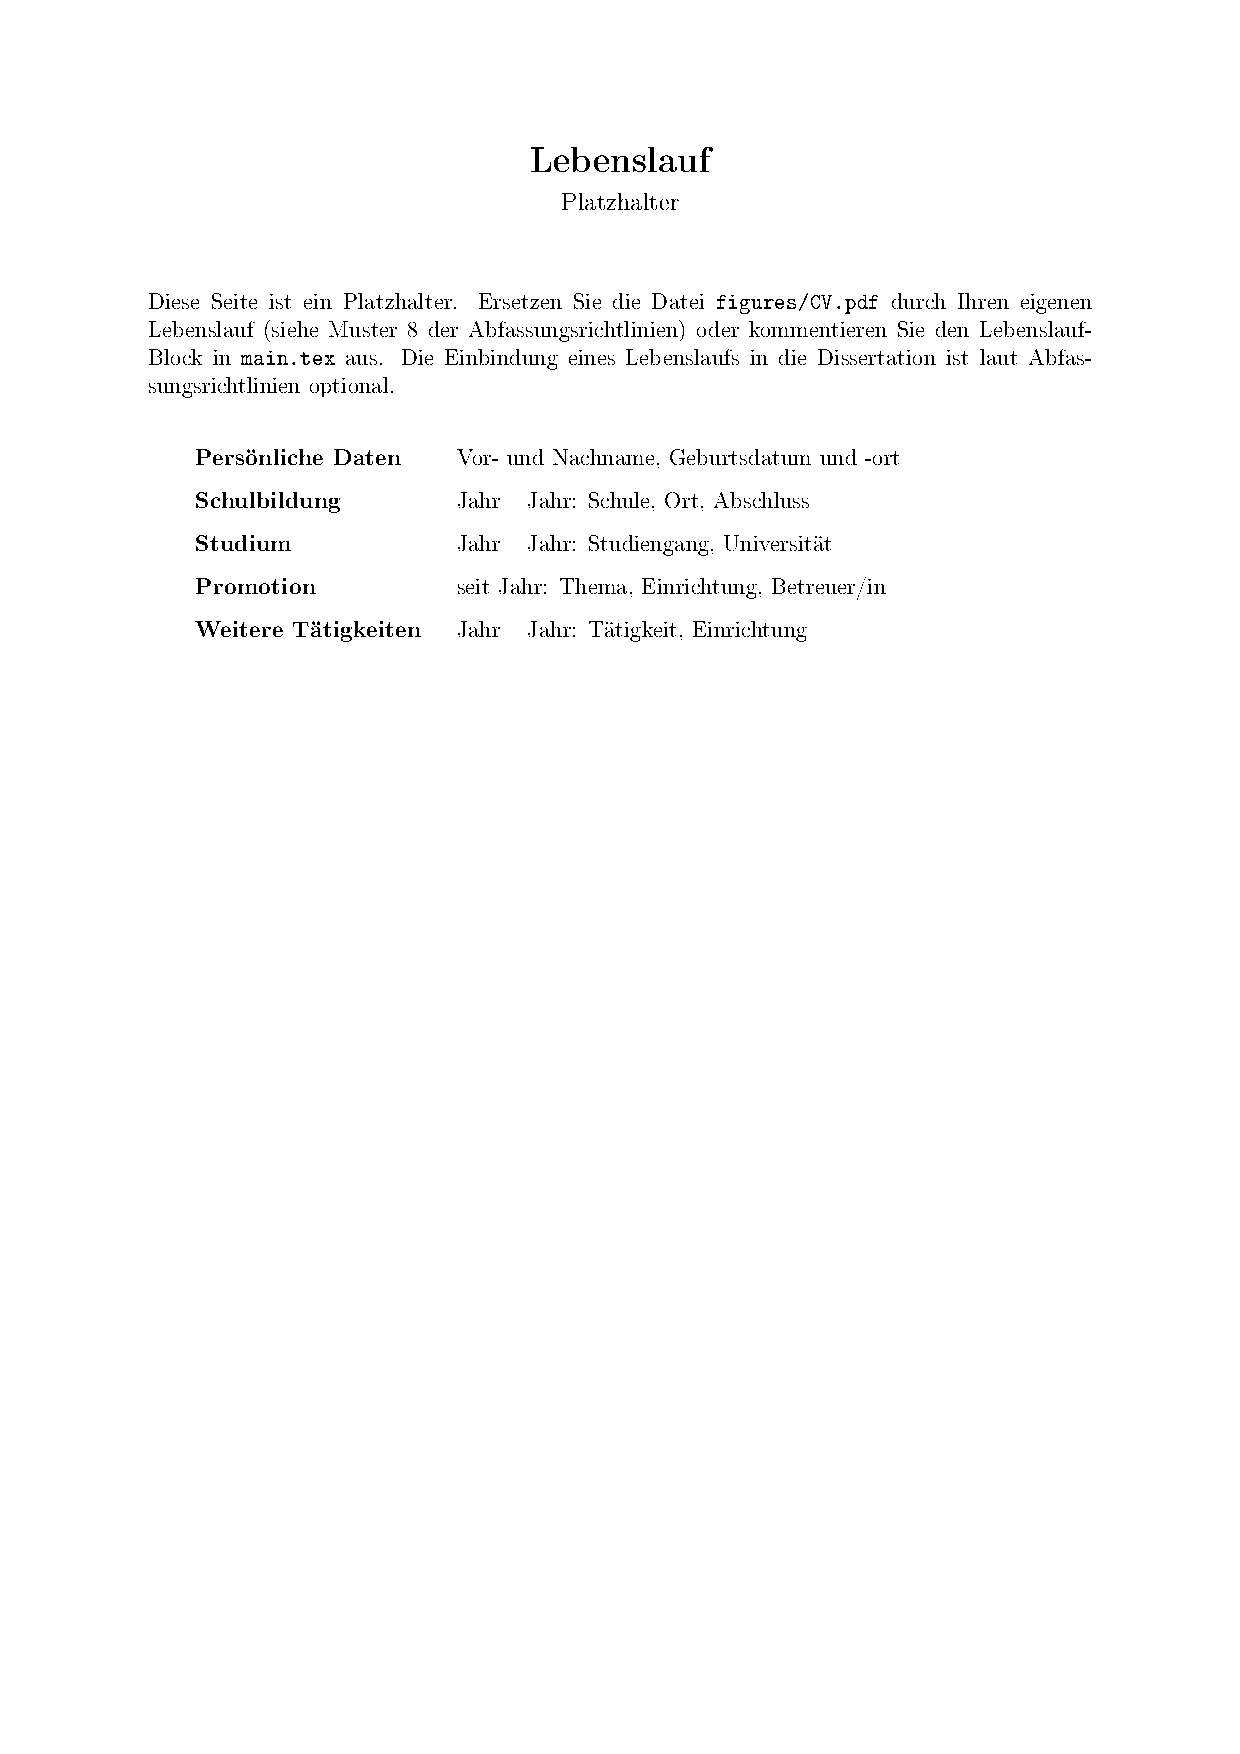
\includepdf[pages=-,frame,scale=.77,pagecommand={\thispagestyle{plain}}]{figures/CV.pdf}

    \chapter*{Acknowledgement}
\addcontentsline{toc}{chapter}{Acknowledgement}

\lipsum[1-3]

    % PFLICHTTEXT (Muster 10 der Abfassungsrichtlinien): Wortlaut nicht umformulieren.
% Muss in deutscher Sprache eingebunden und in allen Pflichtexemplaren
% handschriftlich unterschrieben werden.
% Ausnahme laut Muster 10: Wurden die Arbeit oder Teile davon bereits an einer
% Hochschule als Prüfungs- oder Qualifikationsleistung vorgelegt, ist Punkt 3
% durch die Variante aus Muster 10 zu ersetzen (Titel der Arbeit, Hochschule und
% Jahr, Art der Prüfungs- oder Qualifikationsleistung angeben).
\chapter*{Eidesstattliche Versicherung}
\vspace{-6em}{\Huge\color{dkfzgray2} Statutory Declaration}
\addcontentsline{toc}{chapter}{Eidesstattliche Versicherung (Affidavit) in German}
    
    \begin{enumerate}
        \setlength{\itemsep}{0pt}
        \item Bei der eingereichten Dissertation zu dem Thema \emph{\textbf{\thesistitle}} handelt es sich um meine eigenständig erbrachte Leistung.\\
        \emph{\small\color{dkfzgray2} I herewith formally declare that I have written the submitted dissertation \textbf{\thesistitle} independently.}
        
        \item Ich habe nur die angegebenen Quellen und Hilfsmittel benutzt und mich keiner unzulässigen Hilfe Dritter bedient. Insbesondere habe ich wörtlich oder sinngemäß aus anderen Werken übernommene Inhalte als solche kenntlich gemacht.\\
        \emph{\small\color{dkfzgray2}  I did not use any third party support except for the quoted literature and other sources mentioned in the text. Content from other work, either literally or in content, has been declared as such.}
        
        \item Die Arbeit oder Teile davon habe ich bislang nicht an einer Hochschule des In- oder Auslands als Bestandteil einer Prüfungs- oder Qualifikationsleistung vorgelegt.\\
        \emph{\small\color{dkfzgray2} The thesis has not been submitted to any examination body in this, or similar, form. }
        
        \item Die Richtigkeit der vorstehenden Erklärungen bestätige ich.\\
        \emph{\small\color{dkfzgray2} I confirm the correctness of the aforementioned declarations.}
        
        \item Die Bedeutung der eidesstattlichen Versicherung und die strafrechtlichen Folgen einer unrichtigen oder unvollständigen eidesstattlichen Versicherung sind mir bekannt. Ich versichere an Eides statt, dass ich nach bestem Wissen die reine Wahrheit erklärt und nichts verschwiegen habe.\\
        \emph{\small\color{dkfzgray2} I am aware of the legal consequences of this declaration. To the best of my knowledge I have told the pure truth and not concealed anything.}
    \end{enumerate}
    
    \begin{tabular}{p{3cm}p{5cm}p{4cm}}
          &  & \\
          & & \\
          &Heidelberg, \today & \hrulefill\\
          & & \textit{TODO: name of doctoral student}
    \end{tabular}
    \ifkiverwendet
        % PFLICHTTEXT (Muster 11 a der Abfassungsrichtlinien, Version 2.5): Wortlaut nicht
% umformulieren, insbesondere der Text ab „Mir ist bewusst, dass ...“ bleibt
% unverändert. Muss in deutscher Sprache eingebunden und in allen
% Pflichtexemplaren handschriftlich unterschrieben werden. Die grauen englischen
% Übersetzungen sind nicht Teil des Musters; im Zweifel beim Promotionsbüro
% nachfragen. Das Muster nennt beide Promotionsordnungen, verbunden mit „oder“;
% hier wird über \thesisdegree (main.tex) die zutreffende ausgewählt.
% Wurden keine KI-basierten Hilfsmittel verwendet, gilt stattdessen Muster 12
% (11b_Erklaerung_Nichtverwendung_KI.tex, Schalter \kiverwendetfalse in main.tex).
\chapter*{Angaben zu den verwendeten KI-basierten elektronischen Hilfsmitteln}
\vspace{-6em}{\Huge\color{dkfzgray2} Information on the AI-based tools used}
\addcontentsline{toc}{chapter}{Angaben zu den verwendeten KI-basierten elektronischen Hilfsmitteln}

Zur Dokumentation der verwendeten KI-basierten Hilfsmittel ist der schriftlichen Ausarbeitung ein besonderer Anhang hinzugefügt, der eine Liste und Beschreibung aller dieser Hilfsmittel enthält. Dieser Anhang zur Dokumentation der verwendeten Hilfsmittel erfüllt folgende Kriterien:

\emph{\small\color{dkfzgray2} To document the AI-based tools used, a special appendix has been added to the written report, which contains a list and description of all of these tools. This appendix documenting the tools used meets the following criteria:}

\begin{enumerate}
    \item Auflistung der Ziele, für die die KI-basierten Hilfsmittel in der vorliegenden Arbeit eingesetzt wurden.\\
    \emph{\small\color{dkfzgray2} List of the goals for which the AI-based tools were used in this work.}
    \item Dokumentation der Verwendungsweise der KI-basierten Hilfsmittel.\\
    \emph{\small\color{dkfzgray2} Documentation of how the AI-based tools were used.}
    \item Nennung der Kapitel und Abschnitte der vorliegenden Arbeit, in denen die KI-basierten Hilfsmittel eingesetzt wurden, um Inhalte zu erzeugen.\\
    \emph{\small\color{dkfzgray2} Identification of the chapters and sections of this work in which AI-based tools were used to generate content.}
\end{enumerate}

Der Gebrauch dieser Hilfsmittel inklusive Art, Ziel und Umfang des Gebrauchs wurde mit meinem offiziellen Betreuer / meiner offiziellen Betreuerin \textbf{TODO NAME OF SUPERVISOR} abgesprochen.

\emph{\small\color{dkfzgray2} The use of these aids, including the type, purpose and extent of use, has been agreed with my official supervisor \textbf{TODO NAME OF SUPERVISOR}.}
\newpage
% PFLICHTTEXT aus Muster 11 a bzw. Muster 12 der Abfassungsrichtlinien (Version 2.5),
% von 11_Angabe_KI.tex und 11b_Erklaerung_Nichtverwendung_KI.tex gemeinsam genutzt.
% Wortlaut nicht umformulieren. Die zutreffende Promotionsordnung wird über
% \thesisdegree (main.tex) ausgewählt.
Mir ist bewusst, dass insbesondere der Versuch einer nicht dokumentierten Nutzung KI-basierter Hilfsmittel als Täuschungsversuch zu werten ist:

\emph{\small\color{dkfzgray2} I am aware that in particular the attempt to use AI-based tools without documentation is to be regarded as an attempt at deception:}

\ifdefstring{\thesisdegree}{schum}{%
Gem. § 16 Abs. 2 der Promotionsordnung „Dr. sc. hum.“:
„Ergibt sich vor Aushändigung der Promotionsurkunde, dass der Doktorand / Doktorandin bei einer Promotionsleistung getäuscht hat, so kann der Promotionsausschuss diese Promotionsleistung oder alle bisher erbrachten Promotionsleistungen für ungültig erklären. In besonders schweren Fällen kann der Promotionsausschuss die Annahme als Doktorand / Doktorandin endgültig widerrufen.“

\emph{\small\color{dkfzgray2} According to § 16 paragraph 2 of the doctoral regulations “Dr. sc. hum.”:
“If it emerges before the doctoral certificate is issued that the doctoral candidate has cheated in a doctoral achievement, the doctoral committee can declare this doctoral achievement or all doctoral achievements to date invalid. In particularly serious cases, the doctoral committee can permanently revoke the acceptance as a doctoral candidate.”}
}{%
Gem. § 16 Abs. 2 der Promotionsordnung „Dr. med. / dent.“:
„Ergibt sich vor Aushändigung der Promotionsurkunde, dass der Kandidat/die Kandidatin bei einer Promotionsleistung getäuscht hat, so können einzelne oder alle Promotionsleistungen für ungültig erklärt werden. In schweren Fällen kann die Zulassung zum Promotionsverfahren zurückgenommen werden.“

\emph{\small\color{dkfzgray2} According to § 16 paragraph 2 of the doctoral regulations “Dr. med. / dent.”:
“If it emerges before the doctoral certificate is issued that the candidate has cheated in a doctoral achievement, individual or all doctoral achievements can be declared invalid. In serious cases, admission to the doctoral process can be withdrawn.”}
}


\begin{tabular}{p{3cm}p{5cm}p{4cm}}
      &  & \\
      & & \\
      &Heidelberg, \today & \hrulefill\\
      & & \textit{TODO: name of doctoral student}
\end{tabular}

        \chapter*{Anhang zur Dokumentation der verwendeten KI-basierten Hilfsmittel}
\vspace{-6em}{\Huge\color{dkfzgray2} Appendix documenting the AI-based tools used}
\addcontentsline{toc}{chapter}{Anhang zur Dokumentation der verwendeten KI-basierten Hilfsmittel}
\par\vspace{2em}

% ---------------------------------------------------------------------------
% ANLEITUNG (vor Einreichung löschen):
%
% Aufbau nach Muster 11 b der Abfassungsrichtlinien (Version 2.5). Dieser Anhang
% steht direkt im Anschluss an die Erklärung (11_Angabe_KI.tex). Für JEDES
% verwendete KI-Tool (z. B. Claude Code, ChatGPT, DeepL, Elicit, GitHub Copilot,
% ...) eine eigene Tabellenzeile anlegen:
%   KI-Tool                    Name des Werkzeugs
%   Version                    Modell/Version oder Nutzungszeitraum (z. B. 10.2026)
%   Verwendete Funktionalität  z. B. LLM, systematische Literaturrecherche
%   Nutzungszweck              z. B. Textkorrektur, Ergänzung der manuellen
%                              Literaturrecherche, Konvertierung eines Entwurfs
%   Einsatzbereich             konkrete Kapitel/Abschnitte, nicht "überall"
%   Art der Validierung        wie die Ergebnisse geprüft wurden, z. B.
%                              Diff-Ansicht, manuelle Quellenprüfung in PubMed,
%                              gezielte manuelle Überprüfung, eigene Texterstellung
%
% KI-Anwendungen, die bereits in "Material und Methoden" ausführlich
% beschrieben sind (z. B. KI als Forschungsmethode), brauchen hier nur einen
% Verweis auf das jeweilige Unterkapitel.
%
% Die Zeile zu Claude Code ist bereits vorbereitet, weil diese Vorlage für die
% Arbeit mit Claude Code gedacht ist. Der Absatz unter der Tabelle zur
% Arbeitsumgebung (heidelberg-med-thesis-claude-template) und zum zugrunde
% liegenden LaTeX-Template von Ayala, Kausch, Klein und Thomas ist die nach
% CC BY 4.0 erforderliche Namensnennung und muss erhalten bleiben.
% ---------------------------------------------------------------------------

{\footnotesize
\renewcommand{\arraystretch}{1.3}
\noindent\begin{tabularx}{\textwidth}{@{}*{6}{>{\raggedright\arraybackslash}X}@{}}
\toprule
\textbf{KI-Tool} & \textbf{Version} & \textbf{Verwendete Funktiona\-lität} & \textbf{Nutzungs\-zweck} & \textbf{Einsatz\-bereich} & \textbf{Art der Validierung} \\
\midrule
Claude Code (Anthropic)
  & TODO: Modell und Nutzungs\-zeitraum
  & TODO (z.\,B. LLM-Agent mit Zugriff auf die LaTeX-Projekt\-dateien)
  & TODO (z.\,B. Konvertierung des Entwurfs in die LaTeX-Vorlage, Textkorrektur)
  & TODO (konkrete Kapitel/\-Abschnitte)
  & TODO (z.\,B. Diff-Ansicht jeder Änderung, gezielte manuelle Überprüfung) \\
\midrule
TODO: weiteres Tool & & & & & \\
\bottomrule
\end{tabularx}
}

\bigskip

\noindent Claude Code wurde innerhalb der frei verfügbaren Arbeitsumgebung
„heidelberg-med-thesis-claude-template“ von Peter Maximilian Full
eingesetzt (\url{https://github.com/pmfull/heidelberg-med-thesis-claude-template},
Lizenz CC BY 4.0). Diese stellt die LaTeX-Vorlage dieser Arbeit sowie
projektspezifische Arbeitsanweisungen für Claude Code bereit, die u.\,a. die
Einhaltung der Abfassungsrichtlinien der Medizinischen Fakultät Heidelberg und
der KI-Leitlinie der Universität Heidelberg vorgeben und das Erfinden von
Quellen untersagen, sowie einen Prüf-Agenten, der die Arbeit auf Formvorgaben
und Kohärenz prüft, ohne sie zu verändern. Die LaTeX-Vorlage basiert auf dem
LaTeX-Template von Leonardo Ayala, Lisa Kausch, André Klein und Sarina Thomas
(\url{https://www.overleaf.com/latex/templates/heidelberg-university-medical-faculty-doctoral-thesis/fzxdxksbfqvm},
Lizenz CC BY 4.0).

\emph{\small\color{dkfzgray2} Claude Code was used within the freely available
working environment “heidelberg-med-thesis-claude-template” by Peter
Maximilian Full
(\url{https://github.com/pmfull/heidelberg-med-thesis-claude-template},
licensed under CC BY 4.0). It provides the LaTeX template of this thesis as
well as project-specific instructions for Claude Code that, among other things,
require compliance with the writing guidelines of the Medical Faculty
Heidelberg and the AI guideline of Heidelberg University and prohibit
fabricating sources, and a review agent that checks the thesis for formal
requirements and coherence without modifying it. The LaTeX template is based on
the LaTeX template by Leonardo Ayala, Lisa Kausch, André Klein, and Sarina
Thomas
(\url{https://www.overleaf.com/latex/templates/heidelberg-university-medical-faculty-doctoral-thesis/fzxdxksbfqvm},
licensed under CC BY 4.0).}

    \else
        % PFLICHTTEXT (Muster 12 der Abfassungsrichtlinien, Version 2.5): nur verwenden,
% wenn für die Dissertation KEINE KI-basierten Hilfsmittel verwendet wurden
% (Schalter \kiverwendetfalse in main.tex). Wortlaut nicht umformulieren. Muss in
% allen Pflichtexemplaren handschriftlich unterschrieben werden.
\chapter*{Erklärung über die Nichtverwendung von KI-basierten elektronischen Hilfsmitteln}
\vspace{-6em}{\Huge\color{dkfzgray2} Declaration on the non-use of AI-based tools}
\addcontentsline{toc}{chapter}{Erklärung über die Nichtverwendung von KI-basierten elektronischen Hilfsmitteln}

Ich versichere hiermit, dass ich für die Erstellung der vorliegenden Dissertation keine KI-basierten elektronischen Hilfsmittel verwendet habe.

\emph{\small\color{dkfzgray2} I hereby declare that I did not use any AI-based tools for the preparation of this dissertation.}

% PFLICHTTEXT aus Muster 11 a bzw. Muster 12 der Abfassungsrichtlinien (Version 2.5),
% von 11_Angabe_KI.tex und 11b_Erklaerung_Nichtverwendung_KI.tex gemeinsam genutzt.
% Wortlaut nicht umformulieren. Die zutreffende Promotionsordnung wird über
% \thesisdegree (main.tex) ausgewählt.
Mir ist bewusst, dass insbesondere der Versuch einer nicht dokumentierten Nutzung KI-basierter Hilfsmittel als Täuschungsversuch zu werten ist:

\emph{\small\color{dkfzgray2} I am aware that in particular the attempt to use AI-based tools without documentation is to be regarded as an attempt at deception:}

\ifdefstring{\thesisdegree}{schum}{%
Gem. § 16 Abs. 2 der Promotionsordnung „Dr. sc. hum.“:
„Ergibt sich vor Aushändigung der Promotionsurkunde, dass der Doktorand / Doktorandin bei einer Promotionsleistung getäuscht hat, so kann der Promotionsausschuss diese Promotionsleistung oder alle bisher erbrachten Promotionsleistungen für ungültig erklären. In besonders schweren Fällen kann der Promotionsausschuss die Annahme als Doktorand / Doktorandin endgültig widerrufen.“

\emph{\small\color{dkfzgray2} According to § 16 paragraph 2 of the doctoral regulations “Dr. sc. hum.”:
“If it emerges before the doctoral certificate is issued that the doctoral candidate has cheated in a doctoral achievement, the doctoral committee can declare this doctoral achievement or all doctoral achievements to date invalid. In particularly serious cases, the doctoral committee can permanently revoke the acceptance as a doctoral candidate.”}
}{%
Gem. § 16 Abs. 2 der Promotionsordnung „Dr. med. / dent.“:
„Ergibt sich vor Aushändigung der Promotionsurkunde, dass der Kandidat/die Kandidatin bei einer Promotionsleistung getäuscht hat, so können einzelne oder alle Promotionsleistungen für ungültig erklärt werden. In schweren Fällen kann die Zulassung zum Promotionsverfahren zurückgenommen werden.“

\emph{\small\color{dkfzgray2} According to § 16 paragraph 2 of the doctoral regulations “Dr. med. / dent.”:
“If it emerges before the doctoral certificate is issued that the candidate has cheated in a doctoral achievement, individual or all doctoral achievements can be declared invalid. In serious cases, admission to the doctoral process can be withdrawn.”}
}


\begin{tabular}{p{3cm}p{5cm}p{4cm}}
      &  & \\
      & & \\
      &Heidelberg, \today & \hrulefill\\
      & & \textit{TODO: name of doctoral student}
\end{tabular}

    \fi

\end{document}
